\documentclass[10pt,a4paper,fleqn]{article}
\usepackage[utf8]{inputenc}
\usepackage{amsmath}
\usepackage{amsfonts}
\usepackage{amssymb}
\usepackage[T1]{fontenc}
\usepackage{geometry}
\geometry{a4paper}
\usepackage[english]{babel}
\usepackage{dcolumn}
\usepackage{graphicx}
\usepackage{ntheorem}
\theoremseparator{:}
\newtheorem{theorem}{Hypothesis}
\usepackage{chngcntr}
\newcounter{pretheorem}
\counterwithin{theorem}{pretheorem}
\usepackage{caption}
\usepackage{textcomp}
\usepackage[export]{adjustbox}
\usepackage{float}
\usepackage{grffile}
\usepackage{listings}
\usepackage{fixltx2e}
\usepackage{verbatim}
\usepackage[backend=bibtex, sorting=none]{biblatex}
\usepackage[nottoc,numbib]{tocbibind}
\usepackage{setspace}
\usepackage{relsize}
\usepackage[final]{pdfpages}
\usepackage{wrapfig,lipsum,booktabs}
\usepackage{subcaption}
\usepackage{pdfpages}


\renewcommand\thetheorem{\arabic{pretheorem}\alph{theorem}}
\newcommand{\theoremgroup}{\refstepcounter{pretheorem}}

\renewcommand{\topfraction}{.85}
\renewcommand{\bottomfraction}{.7}
\renewcommand{\textfraction}{.15}
\renewcommand{\floatpagefraction}{.66}
\renewcommand{\dbltopfraction}{.66}
\renewcommand{\dblfloatpagefraction}{.66}
\setcounter{topnumber}{9}
\setcounter{bottomnumber}{9}
\setcounter{totalnumber}{20}
\setcounter{dbltopnumber}{9}


\addbibresource{sample.bib}
\author{Chong Kim}





\begin{document}

\begin{titlepage}
\date{}
	\centering

	{\scshape\LARGE Final Report \par}
	\vspace{1cm}
	{\scshape\Large Asthma Treatment Pattern Longitudinal Analysis \par}
	\vspace{1.5cm}

	\vspace{2cm}
	{\Large\itshape Chong Kim\par}
	\vfill
	supervised by\par
	Dr.~Matthew \textsc{Strand}
	\vfill


	{\large \today\par}

\begin{flushleft}
The Department of Clinical Pharmacy (DOCP) has provided funding for this educational project but has not conducted the
research or written this report. While the authors have worked on the best information available to them, neither
DOBB/DOCP nor the authors shall in any event be liable for any loss, damage or injury howsoever suffered directly or
indirectly in relation to the report or the research on which it is based.
\\~\\
Reference herein to trade names and proprietary products without stating that they are protected does not imply
that they may be regarded as unprotected and thus free for general use. No endorsement of named products is
intended nor is it any criticism implied of other alternative, but unnamed, products.
\end{flushleft}

\end{titlepage}

\newpage
\section{Background and Introduction}

Asthma management guidelines from the American Thoracic Society (ATS) and  the Global Initiative for Asthma (GINA) suggest a stepwise therapeutic management strategy for asthma patients\cite{Bateman2008}. The guidelines suggest that if a patient is not controlled at present time, the lowest possible treatment step should be found such that control is maintained. Operationalization of treatment steps are indicated in Appendix~\ref{ts}.  \\
\indent\textbf{Gap:} Although operationalization of treatment steps have been defined, these treatment patterns' association with patient demographic and clinical characteristics is unknown.\\
\indent In this paper, the association between treatment step patterns and patient characteristics will be examined. Additionally, the association between asthma health outcomes with the treatment step trajectory will be assessed.

\begin{table}[ht]
\centering
\caption{Baseline Characteristics of Study Subjects}
\label{t1}
\resizebox{\columnwidth}{!}{%
\begin{tabular}{rllllllll}
\\[-1.8ex]\hline 
\hline \\[-1.8ex] 
 & \multicolumn{1}{c}{\textit{Baseline Treatment Steps}} \\ 
\cline{2-2} 
  \hline
 & 0 & 1 & 2 & 3 & 4 & 5 & p & test \\ 
  \hline
n & 3896 & 558 & 187 & 182 & 143 & 34 &  &  \\ 
  age (mean (sd)) & 32.19 (18.28) & 28.16 (17.43) & 24.53 (17.25) & 29.25 (18.32) & 34.09 (16.45) & 41.32 (13.84) & $<$0.001 &  \\ 
  Gender (\%) &  &  &  &  &  &  & 0.992 &  \\ 
     F & 2265 (58.0) & 315 (56.5) & 103 (55.1) & 99 (54.4) & 83 (58.0) & 21 (61.8) &  &  \\ 
     M & 1634 (41.9) & 243 (43.5) & 84 (44.9) & 83 (45.6) & 60 (42.0) & 13 (38.2) &  &  \\ 
  pat\_region (\%) &  &  &  &  &  &  & 0.015 &  \\ 
     E & 1115 (28.6) & 149 (26.7) & 56 (29.9) & 37 (20.3) & 34 (23.8) & 13 (38.2) &  &  \\ 
     MW & 1197 (30.7) & 193 (34.6) & 65 (34.8) & 77 (42.3) & 49 (34.3) & 13 (38.2) &  &  \\ 
     S & 1155 (29.6) & 148 (26.5) & 42 (22.5) & 42 (23.1) & 42 (29.4) & 5 (14.7) &  &  \\ 
     W & 429 (11.0) & 68 (12.2) & 24 (12.8) & 26 (14.3) & 18 (12.6) & 3 (8.8) &  &  \\ 
  Insurance (\%) &  &  &  &  &  &  & 0.442 &  \\ 
     1 & 3239 (83.1) & 460 (82.4) & 155 (82.9) & 149 (81.9) & 119 (83.2) & 24 (70.6) &  &  \\ 
     2 & 12 (0.3) & 5 (0.9) & 1 (0.5) & 1 (0.5) & 1 (0.7) & 0 (0.0) &  &  \\ 
     3 & 163 (4.2) & 25 (4.5) & 4 (2.1) & 10 (5.5) & 5 (3.5) & 2 (5.9) &  &  \\ 
     4 & 16 (0.4) & 3 (0.5) & 1 (0.5) & 2 (1.1) & 3 (2.1) & 0 (0.0) &  &  \\ 
     5 & 448 (11.5) & 62 (11.1) & 24 (12.8) & 19 (10.4) & 15 (10.5) & 8 (23.5) &  &  \\ 
     6 & 18 (0.5) & 3 (0.5) & 2 (1.1) & 1 (0.5) & 0 (0.0) & 0 (0.0) &  &  \\ 
  baseline\_cost (mean (sd)) & 2332.40 (8456.03) & 1976.91 (5186.50) & 1627.84 (3147.64) & 2033.80 (6760.94) & 2273.61 (4161.81) & 3005.02 (4810.03) & 0.741 &  \\ 
  CCI (mean (sd)) & 0.29 (0.62) & 0.15 (0.48) & 0.13 (0.43) & 0.20 (0.55) & 0.24 (0.74) & 0.35 (0.65) & $<$0.001 &  \\ 
   \hline
\end{tabular}%
}
\end{table}

\section{Method}
Data is from IMS PharMetrics Plus claims data\cite{LifeLink}. The original data encompasses 55,870 subjects but a random sample of 5,000 subjects were sampled for the analysis. The study period is from January 2006$\sim$December 2013. Patient inclusion/exclusion criteria are indicated in the Appendix~\ref{pc}. The primary outcomes of interest are treatment step(ordinal) and asthma health events categorized as dichotomous and nominally; No event and event (i.e. asthma-related hospitalization, asthma-related emergency department visit, asthma-related outpatient exacerbation, and outpatient visit for lower respiratory infection treated with antibiotics). Specific details of the variables are in the Appendix~\ref{va}. After enrollment into the study (index time), the treatment step changes according to asthma severity. The initial baseline characteristics are indicated in Appendix~\ref{pc}. 
\\
Initial data summary of demographic characteristics were examined to get a sense of the underlying assumptions and trends in the data. Data were modeled using a generalized linear mixed model(GzLMM) framework for both outcomes of interests. A priori selection of covariates of interest were age, gender, charlson comorbidity index (CCI), region and insurance type. \\
\textbf{Treatment Step Outcome Model:} Polynomial effect of time(in years as continuous), from linear to sextic term, were considered for the modeling of the treatment step outcome and up to cubic term for modeling of the asthma exacerbation event. Sensitivity analyses were conducted regarding the addition of polynomial terms and indicated age, year, CCI, and insurance was robust while gender was significant while region became insignificant beyond the quintic term. Random intercept and random slope for year by subject were incorporated. The model utilized a multinomial distribution with a cumulative logit link and assuming a proportional odds\cite{hedeker2008multilevel}. \\
\textbf{Asthma Exacerbation Outcome Model:} Interaction between treatment step by year was included to allow the trajectory of treatment steps to vary over time, whereas for the treatment step outcome interaction term of different covariates by year were considered but not included due to lack of significance. Random intercept and random slope for year by subject were incorporated. Models were chosen based on AIC. A range of covariance structure for the random effects were examined that best describes the correlation of the random effects. Analysis method for exacerbation was done using both a binomial distribution (logit link) and a multinomial distribution (generalized logit link). Data were analyzed using SAS PROC GLIMMIX and R packages 'lme4'. 


\section{Results}
The final model to identify the association between asthma treatment steps and patient characteristics is written as
\begin{flalign}
logit(P(Y_{i}<c)) & = \theta_{c} - \beta_{1}base age_{i} -   \beta_{2}CCI_{i}-  (\beta_{3}+b_{i1})year_{ij}- \beta_{4}Insurance_{i} - \\\nonumber 
& \ gender_{k} - b_{i0} -  \beta_{5}year^{2} - \beta_{6}year^{3} - \beta_{7}year^{4} - \beta_{8}year^{5} - \\\nonumber
& \  \beta_{10}year^{6} \ i=1,..,n; c=1,...,C-1 \ where \ C = 6\ steps; k=1,2;l=1,...,r_{i}; \\\nonumber
 & \ \theta_{j} = Threshold \ variable; \ b \sim N(0,G);\ G \ structure \ VC \nonumber
\end{flalign}
The association between year (including and all higher order polynomial terms for year), age, gender, and CCI were significantly associated with the treatment steps (p<0.05, Appendix~\ref{tsmo}). 

%------------------------------------------
\begin{wraptable}{r}{8cm}
\caption{Proportional Odds of Treatment Step}\label{t2}
\centering
\begin{tabular}{rrlr}
  \hline
 Treatment.Step & P(Y$\geq$x) & P(Y=x) \\ 
  \hline
   5 & 0.0064 & 0.01 \\ 
   4 & 0.0621 & 0.06 \\ 
  3 & 0.1312 & 0.07 \\ 
   2 & 0.2343 & 0.10 \\ 
  1 & 0.3963 & 0.16 \\ 
   0 & 1 & 0.60 \\ 
  & \textbf{SUM} & 1.00 \\ 
   \hline
\end{tabular}
\end{wraptable} 
%------------------------------------------
%------------------------------------------
{With the proportional odds assumption, the odds of patients being in treatment step 0 is the highest (0.60) and being in treatment step 5 is the lowest (0.01) after adjusting for covariates. Over all response levels, 1 year increase showed smaller odds of being in greater treatment steps (1 to 5) by 0.916 times. Similarly, over all response levels, females displayed a smaller odds of being in higher treatment steps by 0.894 times. Although a very small effect, over all response levels, 1 year increase in baseline age showed greater odds of being in greater treatment steps by 1.002 times. Similarly, over all response levels, 1 unit increase in CCI showed greater odds of being in greater treatment steps by 1.053 times. Sensitivity analyses results indicate that after adding the quintic term for year, the association between gender becomes significant (previously not significant) while the effect of region becomes non-significant. The random effects covariance structure was kept as variance component (VC) due to the fact that the AIC for the VC model was better than the unstructured (UN) model.\\~\\
\par
%------------------------------------------

The final model to identify the association between asthma exacerbation events (binary) and asthma treatment steps adjusting for relevant covariates can be written as
\begin{flalign}
\log(\dfrac{p}{1-p}) & = \beta_{0} + \beta_{1}base age_{i} +   \beta_{2}CCI_{i} + \beta_{3}Insurance_{i} + (\beta_{4}+b_{i1})year_{ij}  + \\\nonumber
& \beta_{5}year^{2}_{ij}  + \beta_{6}year^{3}_{ij} + gender_{k} + \beta_{7}TS_{ij} + \beta_{8}TS_{ij}*year_{ij} + b_{i0} \\\nonumber  & i=1,..,n;k=1,2;j=1,...,r_{i}; \nonumber
\end{flalign}

In this model, baseline age and Insurance type was not statistically significantly associated but year (and all polynomial terms for year), treatment step, year by treatment step interaction, gender, region, and CCI were statistically significantly associated (Appendix ~\ref{abmo}). Figure~\ref{fig1} indicates the results from the asthma exacerbation event predicted probabilities by treatment steps. The marginal model that takes into account the population average predicted values (Fig~\ref{fig:f1}) identifies higher probability of event for treatment step 5 and 0 over time compared to the other treatment steps. The conditional model (Fig~\ref{fig:f2}) is displayed to portray the difficulty in identifying any trends regarding subject-specific predicted probabilities of event over time.  


\begin{figure}[!htbp]
  \begin{subfigure}[b]{0.5\textwidth}
    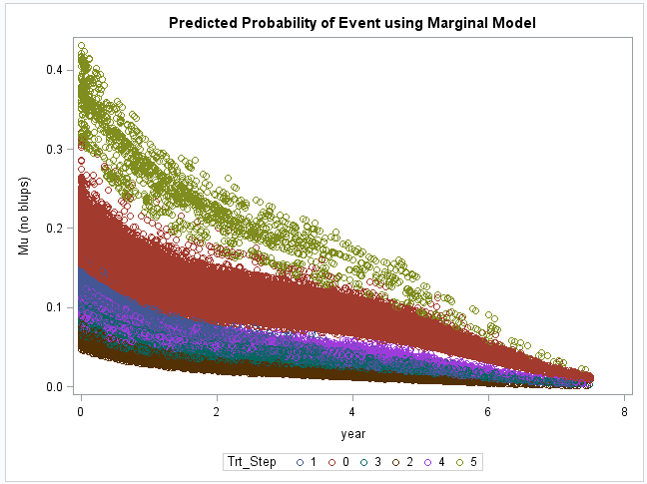
\includegraphics[width=\textwidth]{C:/Users/ck/Dropbox/Academic Coursework/FS2016/Longitudinal/Project/Report/Model/12.2.2016/h2amarginal.png}
    \caption{Marginal Model}
    \label{fig:f1}
  \end{subfigure}
  \hfill
  \begin{subfigure}[b]{0.5\textwidth}
    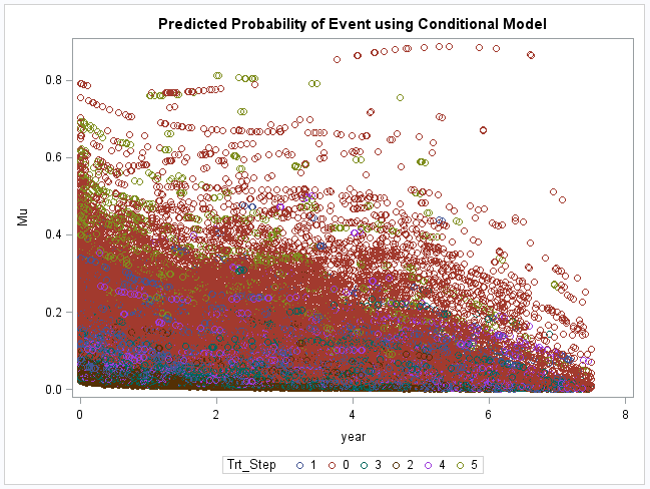
\includegraphics[width=\textwidth]{C:/Users/ck/Dropbox/Academic Coursework/FS2016/Longitudinal/Project/Report/Model/12.2.2016/h2aconditional.png}
    \caption{Conditional Model}
    \label{fig:f2}
  \end{subfigure}
  \caption{Population and Subject-specific Predicted Probabilities of Event by Treatment Step}
  \label{fig1}
\end{figure}


The final model to identify the association between asthma exacerbation events (nominal) and asthma treatment steps adjusting for relevant covariates can be written as
\begin{flalign}
\log(\dfrac{p_{ijc}}{p_{ij1}}) & = \beta_{0} + \beta_{1}base age_{i} +   \beta_{2}CCI_{i} + \beta_{3}Insurance_{i} + (\beta_{4}+b_{i1})time_{ij}  + \beta_{5}time^{2}_{ij}   \\\nonumber 
& + \beta_{6}time^{3}_{ij} +  gender_{k} + \beta_{7}region_{i} + \beta_{8}TS_{ij} + \beta_{9}TS_{ij}*time_{ij} + b_{i0}\\\nonumber
 & \ for \ c=2,3,..,5; \ i=`,..,n;k=1,2;l=1,...,r_{i};) \nonumber
\end{flalign}

The generalized logit model indicates that every variable included is statistically significantly associated with asthma exacerbation event (Appendix~\ref{anmo}). Since the interaction term is significant, compared to no asthma exacerbation event, treatment step 1 subjects have a overall lower odds of asthma exacerbation events (i.e. 0.812 times lesser odds of event 1 compared to event 0) for 1 year increase in time. 
Subjects with 1 unit increase in CCI value have a higher odds of event 1, 3, and 4 (1.157, 1.040, and 1.096 times greater odds) compared to no asthma exacerbation event. Females compared to males had a higher asthma exacerbation event odds compared to no asthma exacerbation event; 1.914 times greater odds of event 1 vs. 0, 1.133 times greater odds of event 2 vs. 0, 1.297 greater odds of event 3 vs. 0, and 1.253 greater odds of event 4 vs. 0. 

\section{Discussion}
From the results indicated for the treatment steps outcome, the reduction in the odds of being in the higher treatment steps for increase in year since diagnosis and being female vs. male while increase in the odds of being in the higher treatment steps for increasing CCI and age units are clear. As indicated in Table~\ref{t2}, the probability of subjects being in higher treatment step is successively smaller which may be a result due to the fact that most asthma patients are in the lower treatment steps or because there are difficulties in capturing the true population of those in higher treatment steps within a claims database. The limitations to the analysis of the treatment steps may be the fact that the proportional odds assumption does not allow for different fixed or random effect slopes for each sub-models (categories of treatment steps). With more powerful (memory efficient) computing facility a nominal mixed model that estimates separate intercept, fixed, and random effects for each sub-model would allow for more flexibility.\\~\\
From the results indicated for the asthma exacerbation events (binary), the plots indicate that the probability of event is highest for those in treatment step 5 and 0 which is also visible in the SAS output. This follows that an asthma exacerbation event for a typical person at one year since diagnosis with an age of 40, male, from region 4, with 1 CCI, and private insurance, in treatment step 5 can be computed as
\begin{flalign}
\eta_{ij} & = -1.5110  -0.5416*1 + 0.1472*1 -0.01720*1 \\\nonumber
& +0.8883 - 0.06917*1 + 0.000998*40 + 0.05947*1 \\\nonumber
& = -1.0343 \\\nonumber
P(Event|\eta_{ij}) & = \dfrac{e^{-1.0343}}{1+e^{-1.0343}} = 0.2623
\end{flalign}
Because asthma exacerbation events are categorized into more categories, we are losing specificity and power regarding estimating each event probability thus we have used the nominal model below.\\~\\
The generalized logit link that allows for the estimation of event probabilities indicate that for the fixed effects, all \textit{a priori} selected covariates displayed significance. In particular, treatment step 5 compared to step 0 with regards to the odds of asthma related outpatient exacerbation (event 3) and Outpatient visit for lower respiratory tract infection (event 4) have a odds of 6.198 and 1.916, respectively after adjusting for covariates. Overall, asthma exacerbation event odds (compared to no event) are decreasing over time for each treatment steps except for slightly higher odds of event 3 for treatment steps 0, 3 and 4. An asthma-related outpatient exacerbation event for a typical person at one year since diagnosis with an age of 40, male, from region 4, with 1 CCI, and private insurance, in treatment step 5 is 0.09259 (calculation described in Appendix~\ref{ev3calc}). As indicated in the calculation and the outputs, the fixed effect and random effect terms for each event (with respect to reference event 0) is estimated separately for each sub-models.\\
Global limitations to each models are that the sample was only a 10\% simple random sample of the whole cohort of the IMS Pharmetrics Asthma population. Also the sampling population was not stratified to include equal allocation of patients within each treatment steps. Even so, the analysis did account for enough subjects within each groups through a simple random sample survey methodology thus we assume the estimation of the fixed and random effects to be robust\cite{brewer1979class}. Adherence measures was not included and may potentially effect the effects of interests\cite{dimatteo2002patient}. Future research should focus on including additional variables that may increase the precision of the effects of interests in this analysis. 

\newpage
\section{Reference}
\printbibliography[title={Articles},type=article,sorting=none,heading=subbibliography]
\printbibliography[title={Books},type=incollection,sorting=none,heading=subbibliography]






\newpage


\section{Appendix}
\subsection{Patient Inclusion/Exclusion Criteria}
\label{pc}
\textbf{Patient entry criteria:}
\begin{enumerate}
  \item evidence of asthma at least two recorded diagnosis for asthma (icd\- 9:493.xx) within 1 year.
  \item having at least 24 months continuous eligibility after index date (follow-up period) and at least 6 months continuous eligibility before index date (pre\- period) environment.
  \item Age 6\- 64 at index.
\end{enumerate}
\textbf{Patient exclusion criteria:}
\begin{enumerate}
  \item diagnosed with cystic fibrosis  (ICD\- 9; 277.0x) or chronic obstructive pulmonary diseases (491.xx, 492.xx, 494.xx and 496.xx) or respiratory tract cancer (160.xx \- 164.xx or 231.xx) or bronchopulmonary dysplasia (770.7x) or respiratory distress syndrome (769.xx).
  \item one of the following diagnoses: Addison disease (255.4x), glomerulonephritis (580.xx to 582.xx), multiple sclerosis (340.xx), polymyositis/dermatomyositis (710.3x, 710.4x), rheumatoid arthritis (714.xx), scleroderma (710.1x), Sjogren disease (710.2x ), systemic lupus erythematosus (710.0x), uveitis (360.11, 363.20 364.3x ), vitiligo (709.01), Wegener granulomatosis (446.4x), Primary systemic vasculitis (447.6x), Crohn?s disease (555.0x to 555.2x, 555.9x), Ulcerative colitis (556.0x to 556.6x, 556.8x, or 556.9x), Chronic eosinophilic pneumonia (518.3x), Idiopathic pulmonary fibrosis (516.3x or 515.xx), minimal change disease (581.3x), autoimmune hepatitis (571.42), Myasthenia Gravis (358.0x), Muscular dystrophy (359.0x, 359.1x, or 359.21), Still?s disease (714.2x), Churg Strauss syndrome (446.4x), Polymyalgia rheumatica (725.xx)
\end{enumerate}
\textbf{Index date:} The first date of asthma diagnosis with 6 months eligibility before the index date (NOTE: asthma diagnosis can occur prior to the index date, however, these diagnoses would not have 6 months eligibility prior to the dates.) \\~\\

\subsection{Variables}
\label{va}
\textbf{Outcomes:}
The primary outcome of interest is a nominal variable that includes:
\begin{enumerate}
  \item No event.
  \item Asthma-related hospitalization.
  \item Asthma-related emergency department visit.
  \item Asthma-related outpatient exacerbation.
  \item Outpatient visit for lower respiratory tract infection treated with antibiotics. 
\end{enumerate}

(See codes and definition in excel)
For patients who have at least one event, we would like to have data on type of event in numeric format and number of days after the index date in numeric format. For those patients with at least one event, only the event category that are observed need to be included i.e. patients who have hospitalization and outpatient exacerbation would only have event 1 and 3 included in the outcome file.
For patient who do NOT have any events during the follow-up time, we would like to include them and have event = 0 and date = missing. 


\textbf{Exposure Variable:}
The primary exposure variable is treatment steps which is an ordinal variable characterized as:
\begin{figure}[!htbp]
\caption{Treatment Step Operationalization}
\label{ts}
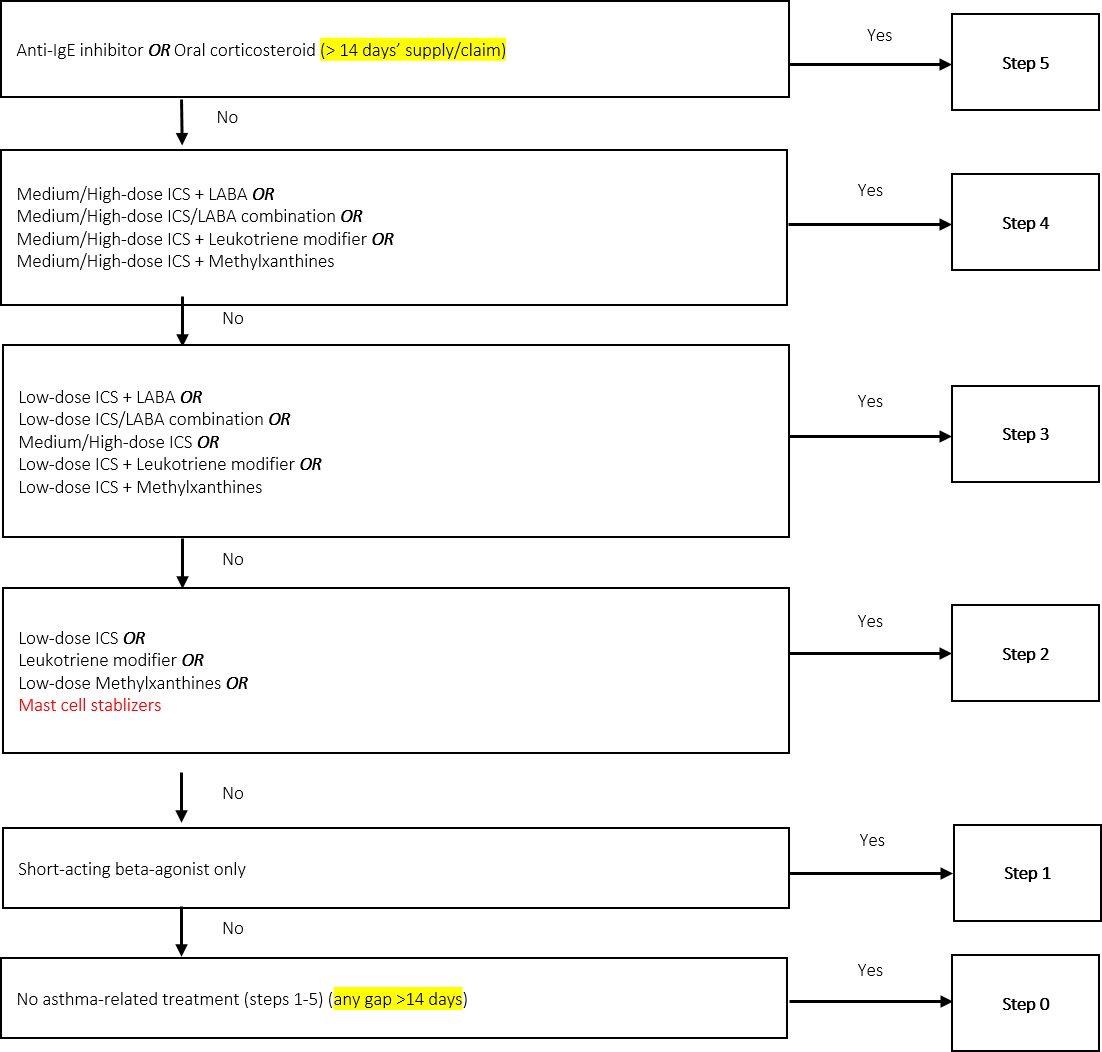
\includegraphics[scale=0.90]{C:/Users/ck/Dropbox/Academic Coursework/FS2016/Longitudinal/Project/Report/trt_step.png}
\end{figure}
\newpage

\subsection{Result}
\subsubsection{Treatment Step Outcome Model Code and Output}
\label{tsmo}
\begin{lstlisting}
proc glimmix data=ats5k method = laplace;
class pat_id region trt_step gender (ref=first) Insurance (ref=first) ;
model trt_step(desc) = year year*year year*year*year year*year*year*year
year*year*year*year*year year*year*year*year*year*year 
age gender region cci insurance / cl dist=multinomial 
link=cumlogit solution oddsratio ;
random int year / subject=pat_id;
run;
\end{lstlisting}

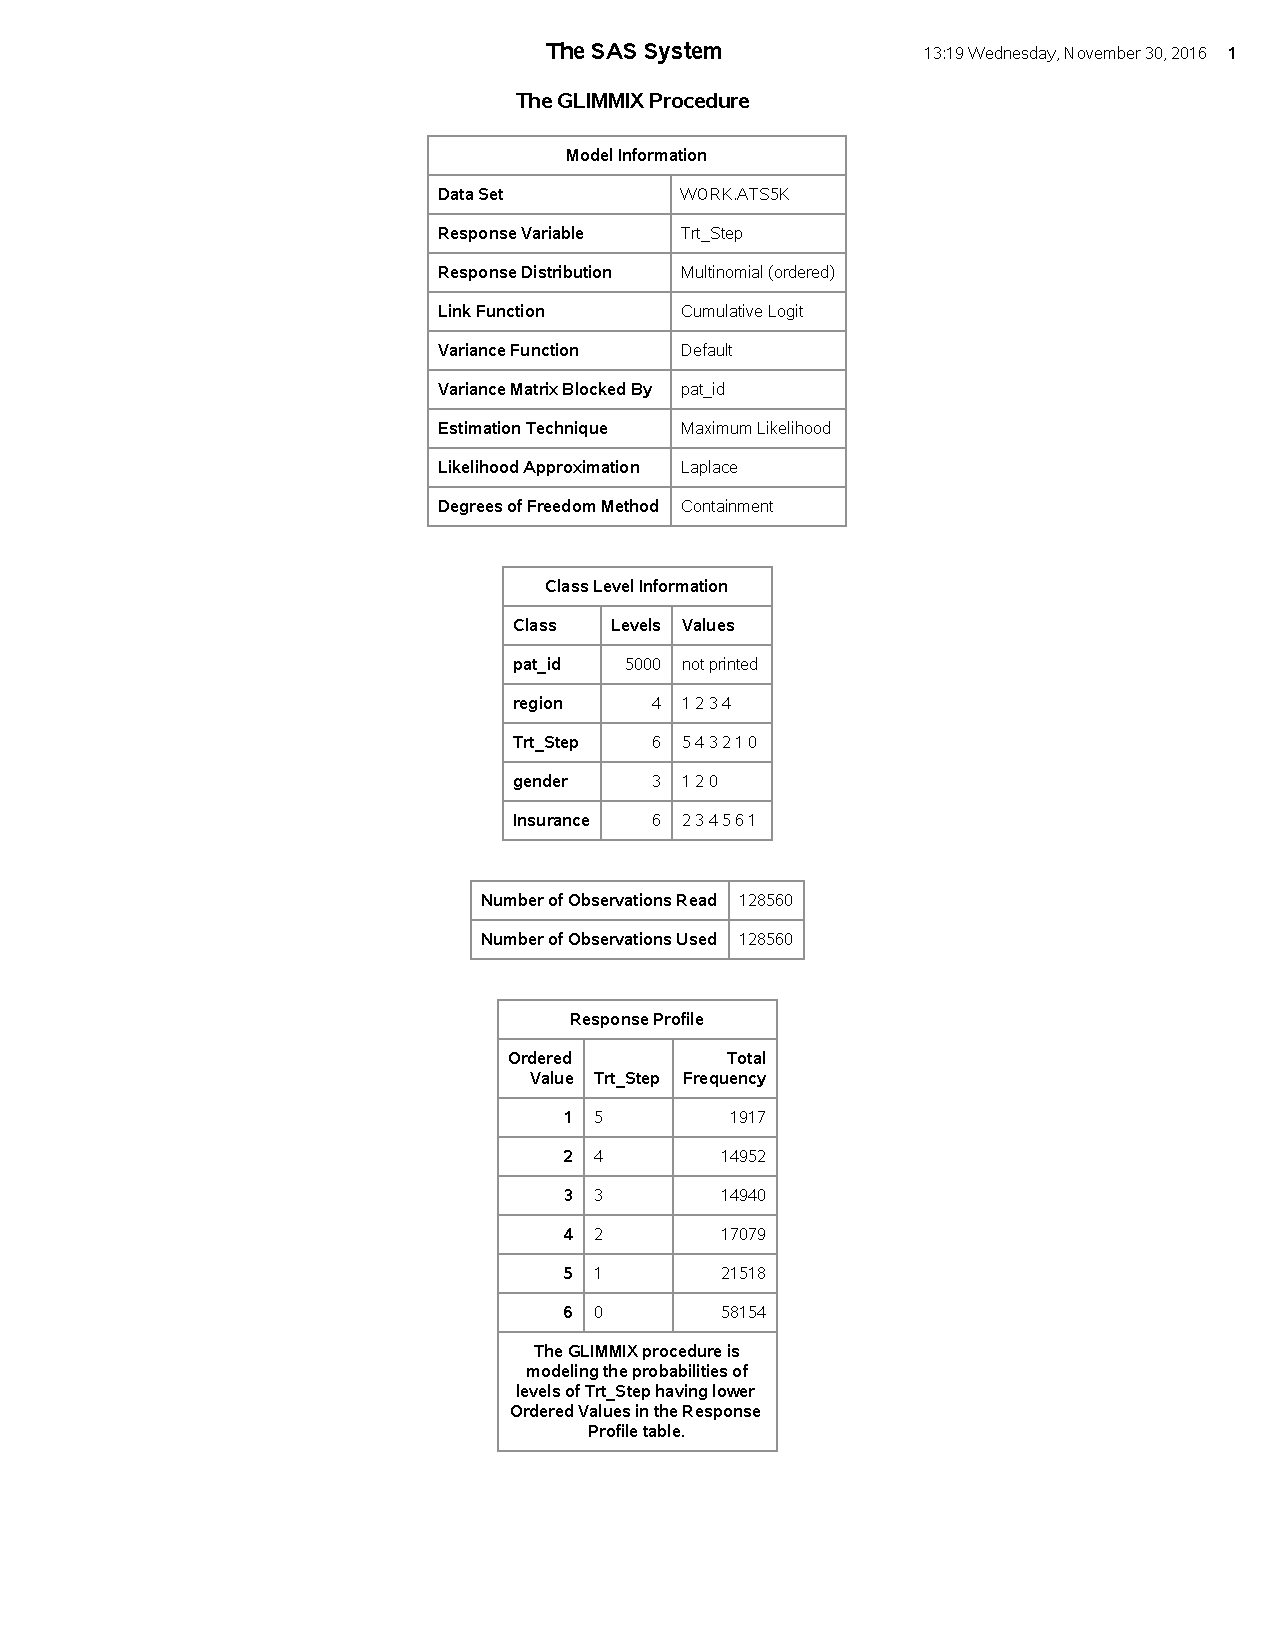
\includepdf[pages={1-},scale=0.75]{C:/Users/ck/Dropbox/Academic Coursework/FS2016/Longitudinal/Project/Report/Model/12.2.2016/H15k.pdf}


\subsubsection{Asthma Exacerbation Outcome (Binary) Model Code and Output}
\label{abmo}

\begin{lstlisting}
proc glimmix data=ats5k method=laplace;
class pat_id region trt_step (ref=first) gender (ref=first) Insurance (ref=first);
model eventb(descending)= year year*year year*year*year trt_step year*trt_step 
age gender region cci insurance / cl dist=binary link=logit solution oddsratio;
random intercept year / subject=pat_id type=vc;
output out=glimmixout 	pred( blup ilink)=PredProb
						pred(noblup ilink)=PredProb_PA
						lcl( blup ilink)=lclpp
						lcl(noblup ilink)=lclpp_pa
						ucl( blup ilink)=uclpp
						ucl(noblup ilink)=uclpp_pa
;
run;
\end{lstlisting}

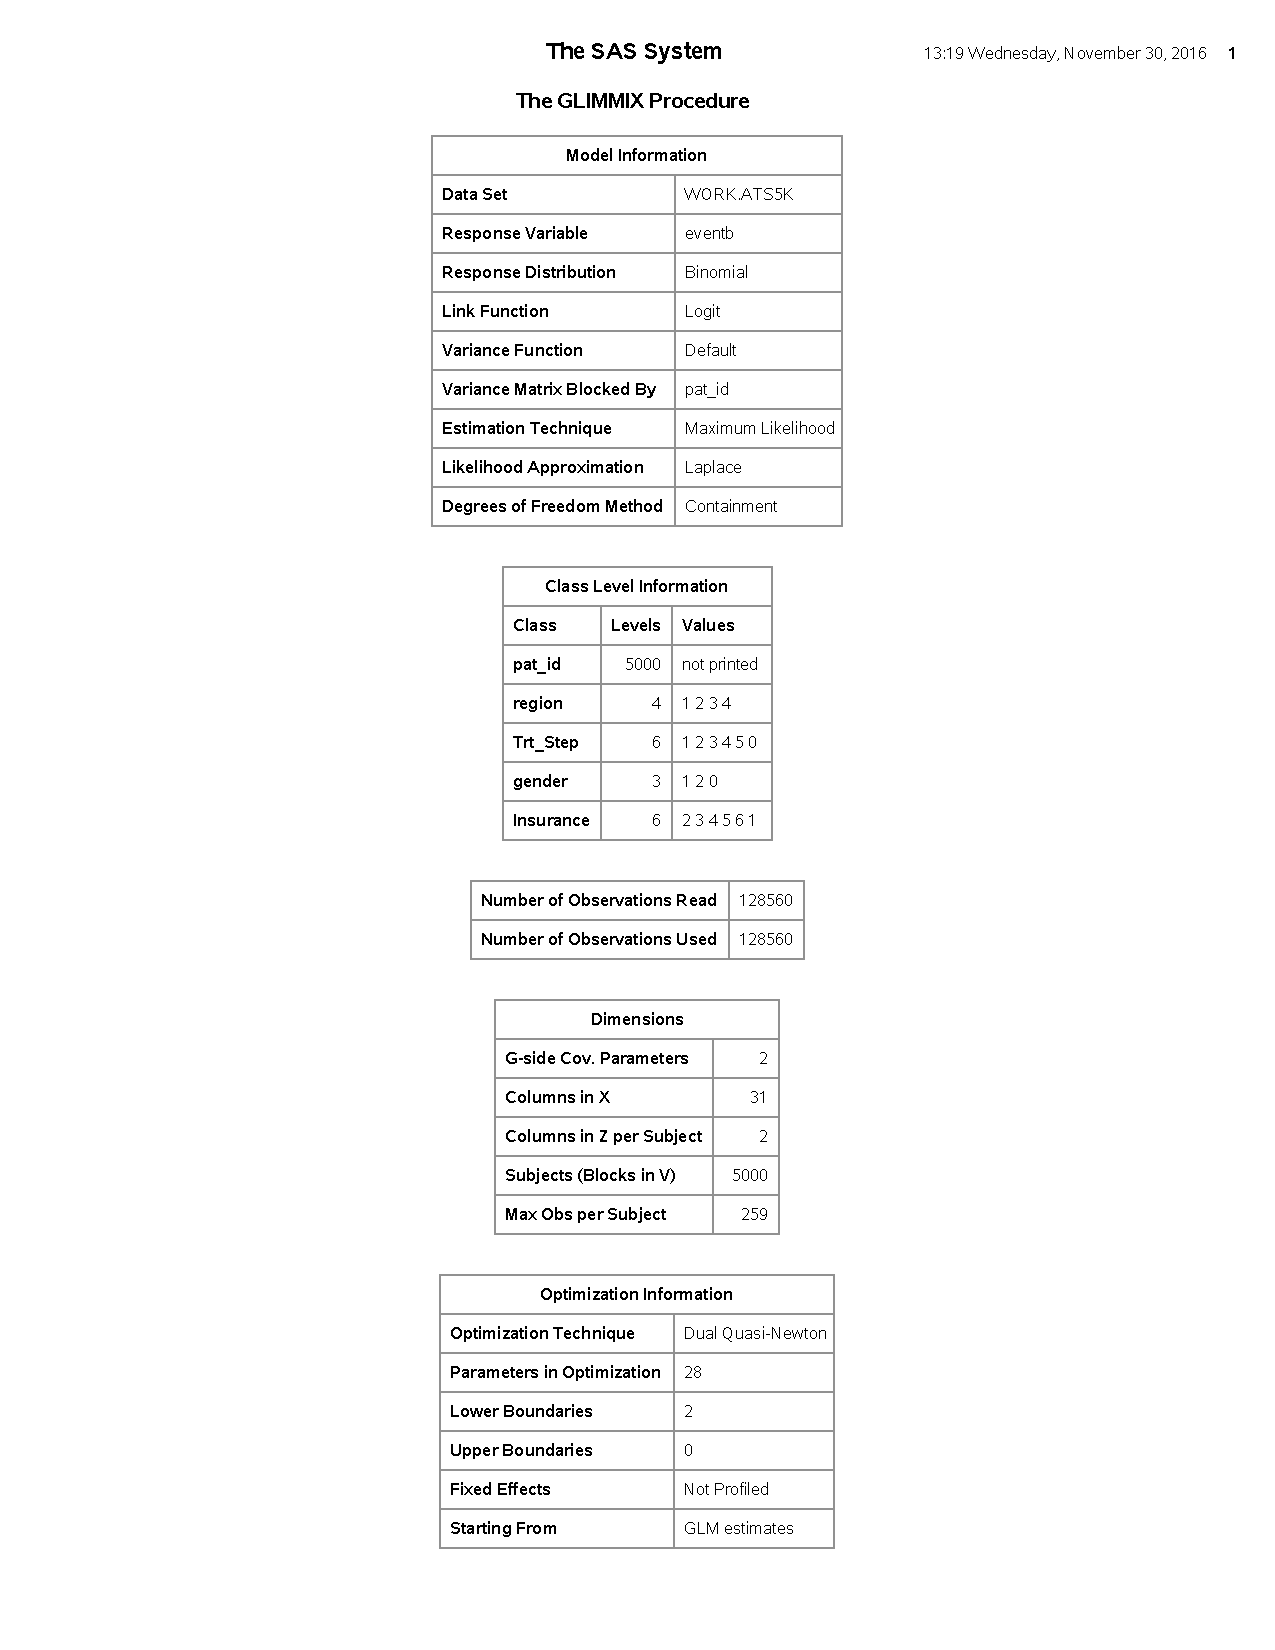
\includepdf[pages={1-},scale=0.75]{C:/Users/ck/Dropbox/Academic Coursework/FS2016/Longitudinal/Project/Report/Model/12.2.2016/H2a5k.pdf}


\subsubsection{Asthma Exacerbation Outcome (Nominal) Model Code and Output}
\label{anmo}

\begin{lstlisting}
proc glimmix data=ats5k method=laplace;
class pat_id region trt_step (ref=first) gender (ref=first)
 Insurance (ref=first) event(ref=first);
model event(event=first)= year year*year year*year*year trt_step 
year*trt_step age gender cci / cl dist=multinomial link=glogit solution oddsratio;
random intercept / subject=pat_id type=vc group=event;
output out=glimouth2	pred( blup ilink)=PredProb
						pred(noblup ilink)=PredProb_PA;
run;
\end{lstlisting}


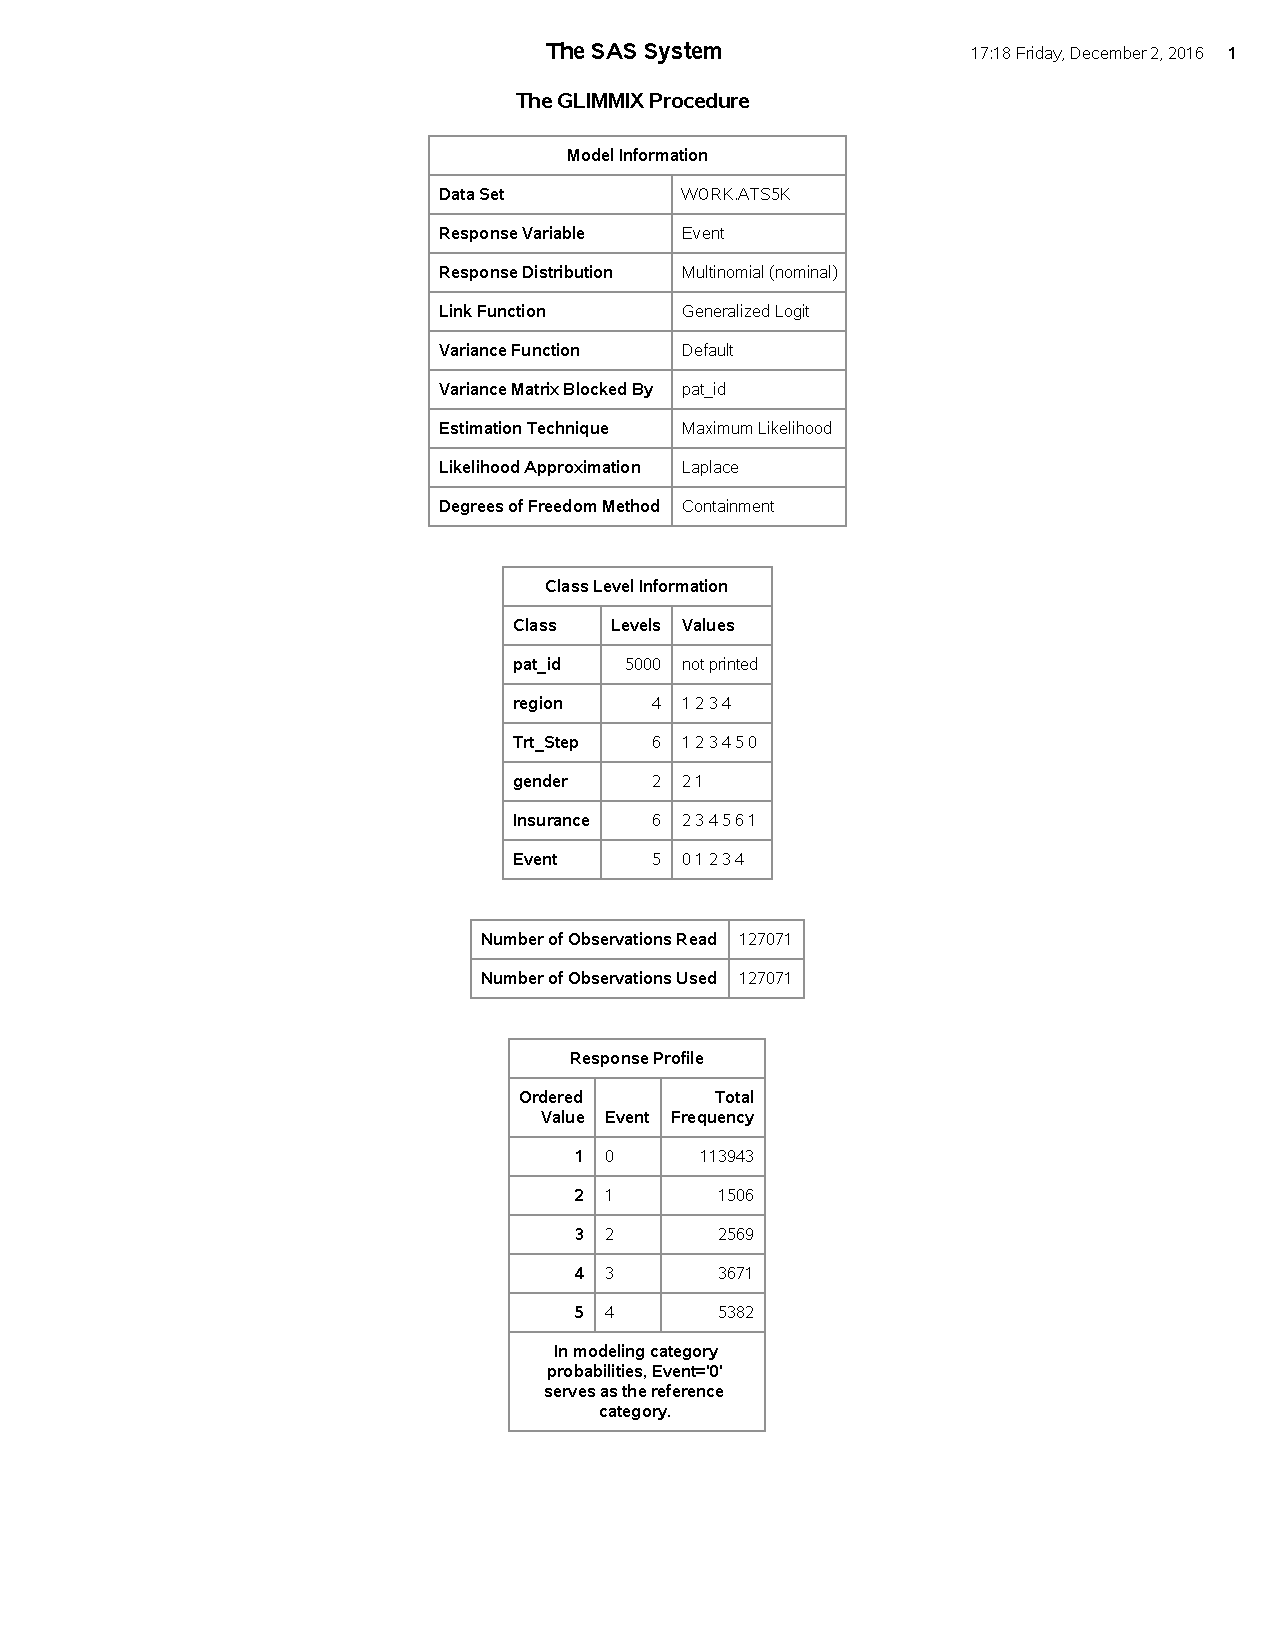
\includepdf[pages={1-},scale=0.75]{C:/Users/ck/Dropbox/Academic Coursework/FS2016/Longitudinal/Project/Report/Model/12.2.2016/H2mn5k.pdf}

\subsubsection{Marginal and Conditional Model Predicted Probability Graph}
\label{ppg}

\begin{lstlisting}
title 'Predicted Probability of Event using Marginal Model';
proc sgplot data=glimmixout;
	scatter x=year y=PredProb_PA / group=trt_step;
run;

title 'Predicted Probability of Event using Conditional Model';
proc sgplot data=glimmixout;
	scatter x=year y=PredProb / group=trt_step;
run;
\end{lstlisting}


\subsubsection{Asthma Exacerbation Outcome (Nominal) Model Exacerbation Event 3 Probability Calculation}
\label{ev3calc}
\begin{flalign}
z_{ij1} & = -6.2847  - 0.3169*1 - 0.1027*1 + 0.006715*1 \\\nonumber
& - 1.4323 - 0.03979*1 + 0.02322*40 + 0.1460*1 \\\nonumber
& = -7.09488 \\\nonumber
z_{ij2} & = -2.4067  - 0.6361*1 + 0.1202*1 - 0.01051*1 \\\nonumber
& - 0.8141  - 0.07828*1 - 0.00441 *40 - 0.02623*1 \\\nonumber
& = -4.02812 \\\nonumber
z_{ij3} & = -3.5684  - 0.8306*1 + 0.2922*1 -0.02812*1 \\\nonumber
& + 2.0221 - 0.1085*1 - 0.00011*40 + 0.03921*1 \\\nonumber
& = -2.18651 \\\nonumber
z_{ij4} & = -2.7509   - 0.6793*1 + 0.2217*1 -0.02249*1 \\\nonumber
& + 0.7649 - 0.06279*1 - 0.00160 *40 + 0.09205*1 \\\nonumber
& = -2.50083 \\\nonumber
P(Event=3|z_{ij}) & = \dfrac{e^{-2.18651}}{1+e^{-2.18651}+e^{-7.09488}+e^{-4.02812}+e^{-2.50083}} = 0.09259
\end{flalign}



\end{document}